 \documentclass{article}

% Gestion des fonts
\usepackage[utf8]{inputenc}
%\usepackage[T1]{fontenc}

% Langue de rédaction
\usepackage[french]{babel}

% Gestion des images
\usepackage{graphics}
\graphicspath{{./img/plot/},{./img/screenshot/}}
\DeclareGraphicsExtensions{.pdf,.png,.jpg}

% Gestion de l'esthètique
\usepackage[textwidth=0.7\paperwidth, textheight=0.7\paperheight]{geometry}

% Gestion des espaces
\usepackage{xspace}

% Commandes utilisateurs
\newcommand{\alinea}{\setlength{\parindent}{1cm}}
\newcommand{\abaqus}{\bsc{Abaqus}\xspace}
\renewcommand{\listfigurename}{Liste des figures}
% Bibliographie
% \bibitem[label 1]{cle 2} Auteur 3, TITRE 4, editeur 5, annee 6
\renewcommand{\bibitem}[6]{\bibitem[#1]{#2} \textsc{#3}, \emph{#4}, #5, #6}


% Page de garde
\title{Compte-rendu du BE Butée offshore}
\author{\bsc{Muller} Marc \and \bsc{Buquet} Joseph}

\begin{document}
Rapport
\section{Abstract}

\section{Introduction}

%TODO Unités utilisées
% cm ^= 10 k Pa

%TODO Justification de la raideur transverse
% Explication de l'isogonflement lors de l'ajout de rondelles de métal

%TODO Raideur initiale
% Objectif 954 x 4 = 3816 N/cm

%TODO Justification choix lamelle
% Rayon identique à l'élastomère ou supérieur

\section{Approche du problème}

\begin{tabular}{|l|c|}
\hline
Unités & Dimensions \\ \hline
Longueur & cm \\
Pression & k Pa \\
Force & N \\
Raideur & N\/cm \\ \hline
\end{tabular}

\subsection{Butée offshore}
% taille, forme
% compression
% materiau
La butée offshore étudiée est une butée cylindrique de rayon $R_0 = 70 cm$ et de hauteur $H_0 = 100 cm$ en Chloroprène X10. Dans le cadre de cette étude, la butée va être soumise à une compression afin d'évaluer sa raideur à une flèche de $\Delta H = 30 cm$.

Pour ce faire, une modélisation numérique de celle-ci va être faite sous \abaqus. Dans ce contexte, les hypothèses suivantes seront avancées :
\begin{itemize}
\item Matériau isotrope
\item Symétrie axiale
La géométrie axiale de la pièce est cylindrique. Le matériau est de plus isotrope. Enfin la contrainte de compression se fait parallèlement à l'axe de symétrie de la pièce, elle valide donc l'utilisation de symétrie axiale.
\item Modélisation du matériau
\end{itemize}

\subsection{Choix des paramètres de Mooney-Rivlin}
% Les notres : C10 0.2499 C01 0.0942 D1 0.0584
% Les siennes: C10 0.043  C01 0.495  D1 0.000658
% Détails de la manip sur Abaqus + explication MR


%TODO Définition du potentiel élastique...
Description de la méthode de Mooney-Rivlin

La méthode de Mooney-Rivlin est une méthode permettant de modéliser le potentiel de l'énergie de contrainte d'un matériau. Pour cela, il est établi une relation entre le travail du matériau et les invariants $I_1$,$I_2$,$I_3$ définit tel que $I_1 = Trace(\sigma)$, $I_2 = \sec(\sigma)$, $I_3=\det(\sigma)$.
La méthode de Mooney-Rivlin définit en 1940(Mooney) statue la relation suivante : $W = C_10(I_1-3) + C_01(I_2-3) + C_11(I_1-3)(I_2-3)$.

Le modèle de Mooney-Rivlin peut être vu comme un cas particulier du modèle Ogden.

On remarque que l'invariant $I_3$ n'est pas compris dans ce modèle. En effet, pour les élastomères, nous travaillons avec un effet Poisson $\nu = 0.49$, c'est-à-dire à volume quasi-constant. L'invariant $I_3$ est donc égal à 1 et n'est donc pas intéressant pour la modélisation de notre matériau.

\subsection{Contact}
Lors de la compression de la butée offshore, il peut arriver que deux parties de l'élastomère rentrent en contact. Dans ce cas, il faut définir des lois de contacts pour les gérer. 

\subsection{Choix du maillage}

\subsection{calcul de la raideur}

La raideur caractérise la résistance à la déformation élastique d'un corps, c'est-à-dire la la valeur d'effort à lui appliquer pour engendrer une déformation donnée. Dans notre cas, le déplacement est imposé, et la simulation \abaqus nous fournit la force de réaction selon l'axe $\vect{y}$. La raideur $k$ de la butée offshore s'exprime ainsi:
\begin{displaymath}
		k=\frac{F_{y}}{y}
	\end{displaymath}
avec $y$ le déplacement axial imposé en compression et $F_{y}$ la force de réaction axiale associée à celui-ci. 

Dans l'ensemble de l'étude, la raideur $k$ sera caractérisée pour un déplacement de 30cm afin de pouvoir comparer celle-ci à la raideur des autres modèles proposés. Comme il n'y a pas de vibrations d'amplitude de déplacement autour d'une valeur quelconque dans ce cas, la raideur correspondra à la pente de la droite reliant l'origine et le point maximal de la courbe de force-déplacement générée par la simulation \abaqus, c'est-à-dire calculée comme suit:
\begin{displaymath}
		k=\frac{F_{y,max}}{30}
	\end{displaymath}
$k$ a pour unité XXXXXXXXXXXXX.


\subsection{Influence du maillage}

L'étude de la butée offshore a débuté par une étude de l'influence du maillage pour associer un maillage idéal à la pièce dans la modélisation \Abaqus. Ainsi, plusieurs simulations de compression ont été effectuées avec la butée initiale (voir section suivante, butée simple dans élements raidisseurs additionnels) pour différents paramètres de maille décroissants du plus grossier au plus fin: 4, 3, 2 et 1cm de largeur.
Une comparaison a consisté à comparer les courbes force-déplacement associés à chacun des maillages pour discerner leurs différences et ainsi leur influence sur les résultats de la simulation en compression. La figure~\ref{fig:fig1} présente les réponses force-déplacement associées à plusieurs taille d'éléments S4R (de forme quadratique avec intégration réduite).

\begin{figure}[!h]
	\centering
	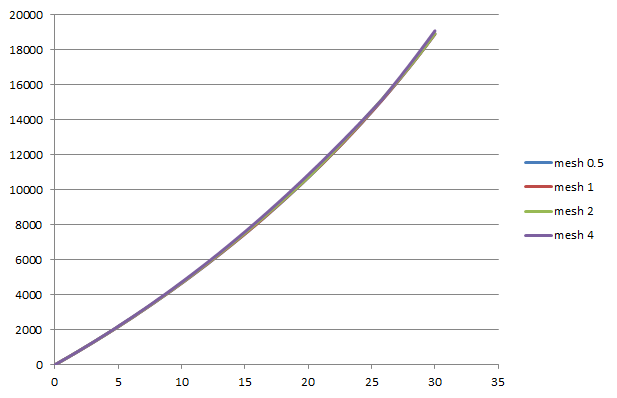
\includegraphics[width=\textwidth]{comparaison_mesh}
	\caption{Réponse force-déplacement de la butée pour différentes tailles de maille.}
	\label{fig1}
\end{figure}

On constate à première vue aucune différence entre les différentes courbes et par conséquent entre les différents maillages. Quand on zoom pour regarder précisément la valeur maximale de la force de réaction pour une flèche de 30cm, comme sur la figure~\ref{fig:fig1}, on constate une lègère différence de 150XXX, c'est-à-dire de 0.8\%, entre un maillage de 4 et 2cm. Un pour un paramètre de maille plus fin, la valeur maximale de la force de réaction converge vers une même valeur.

\begin{figure}[!h]
	\centering
	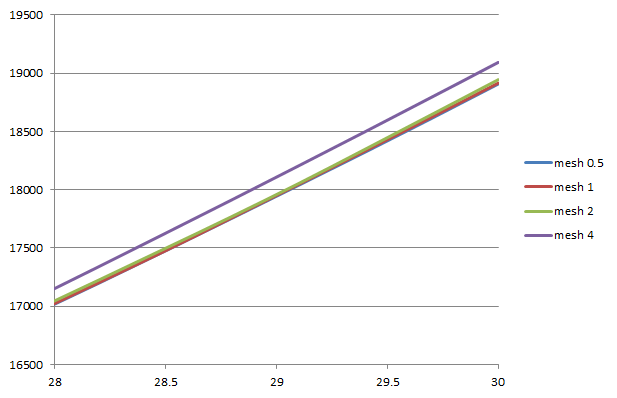
\includegraphics[width=\textwidth]{comparaison_mesh_zoom}
	\caption{Réponse force-déplacement de la butée pour différentes tailles de maille - Zoom.}
	\label{fig1}
\end{figure}

La finesse du maillage n'a donc que très peu d'influence dans notre étude de la raideur de la butée. Un maillage de base d'élements de 2cm de largeur a été cependant choisi pour limiter le temps de calcul, bien qu'un maillage plus fin soit nécessaire dans beaucoup des modèles proposés où le contact avec les pièces additionneles est crutial.


\section{Butée initiale}

L'objectif de cette première partie de l'étude est de décrire le comportement en compression d'une butée offshore en élastomère libre de tout autre élément ou contrainte, afin de rendre compte de la raideur axiale de la pièce et ainsi pouvoir la comparer avec la raideur des autres modèles présentés dans la suite de l'étude.

La forme et le matériau de la butée ainsi que le déplacement imposé à ce dernier ont été décrits dans l'approche du problème. Les élements du maillage dont en S4R et ont pour paramètre 2mm. 



\section{Butée raidie par des lamelles}

\subsection{Lamelles imbriquées}

\subsection{Lamelles larges}
%changement des paramètres de contact -> penalty avec k=10

\subsection{Influence de l'épaisseur des lamelles}
%àfaire


\section{Butée raidie par des anneaux}
%constraint coupling entre le point intérieur de la rondelle et le point exterieur de la butée
%self_contact aussi après


\section{Conclusion}

\listoffigures

\begin{bibliography}{9}
%\bibitem{latexpratique} Christian \textsc{Rolland}. \emph{\LaTeX{} par la pratique}. O'Reilly, 1999.
%\bibitem[label]{cle} Auteur, TITRE, editeur, annee
%\bibitem{label 1}{cle 2}{Auteur 3}{TITRE 4}{editeur 5}{annee 6}
\bibitem{msc}{mcstest}{MSC}{Nonlinear finite elements analysis of elastomers}{MSC Software}{20XX}

% MSC Software, Nonlinear finite elements analysis of elastomers, MSC, 
% CONTACT_SEMINAR page 259
% Mooney Rivlin
%https://en.wikipedia.org/wiki/Mooney%E2%80%93Rivlin_solid
\end{bibliography}
\end{document}
% TOREAD http://www.continuummechanics.org/mooneyrivlin.html
% TOREAD http://dmm.im.ufrj.br/~liu/Papers/MooneyRivlin.pdf
